\documentclass{bredelebeamer}
%%%%%%%%%%%%%%%%%%%%%%%%%%%%%%%%%%%%%%%%%%%%%%%%

\title[每周讨论]{Ways approaching RCP}
\subtitle{''a disordered analog'' of the
Kepler conjecture}
% Sous-titre optionnel

\author{黄朝晖\inst{1}}
% La commande \inst{...} Permet d'afficher l' affiliation de l'intervenant.
% Si il y a plusieurs intervenants: Marcel Dupont\inst{1}, Roger Durand\inst{2}
% Il suffit alors d'ajouter un autre institut sur le modèle ci-dessous.

\institute[北京大学]
{
  \inst{1}%
  力学与工程科学系 \quad 北京大学
}

\date{2021.09.02}

\subject{Sujet de votre diaporama}
% C'est utilisé dans les métadonnes du PDF

\logo{

\includegraphics[scale=0.15]{images/logo.png}
}



%%%%%%%%%%%%%%%%%%%%%%%%%%%%%%%%%%%%%%%%%%%%%%%%%%%%%%%%%%%%%%%%%%%%%
\begin{document}

\begin{frame}
  \titlepage
\end{frame}


\begin{frame}{Outline}
  \tableofcontents
  % possibilité d'ajouter l'option [pausesections]
\end{frame}




\section{Random organization (随机组织)}
\begin{frame}{References 01}
\centerline{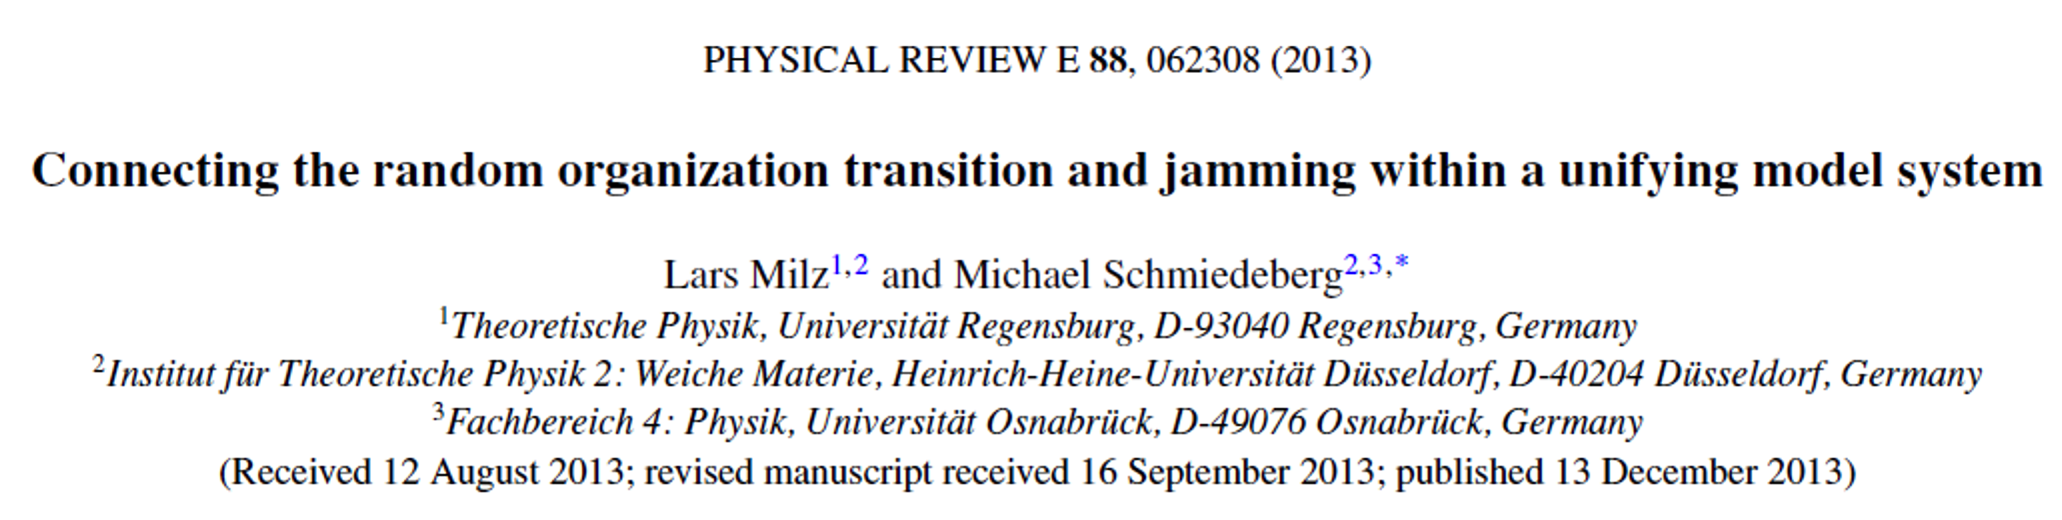
\includegraphics[scale=0.2]{images/p1.png}}
Abstract:
\begin{enumerate}[]
\item The random organization transition + the athermal jamming transition: $\textbf{both
occur within the same model packing problem}$.
\item Our results show that random organization and jamming are $\textbf{opposite limits of
random sphere packings}$.
\end{enumerate}
\end{frame}

\begin{frame}{References 02}
\centerline{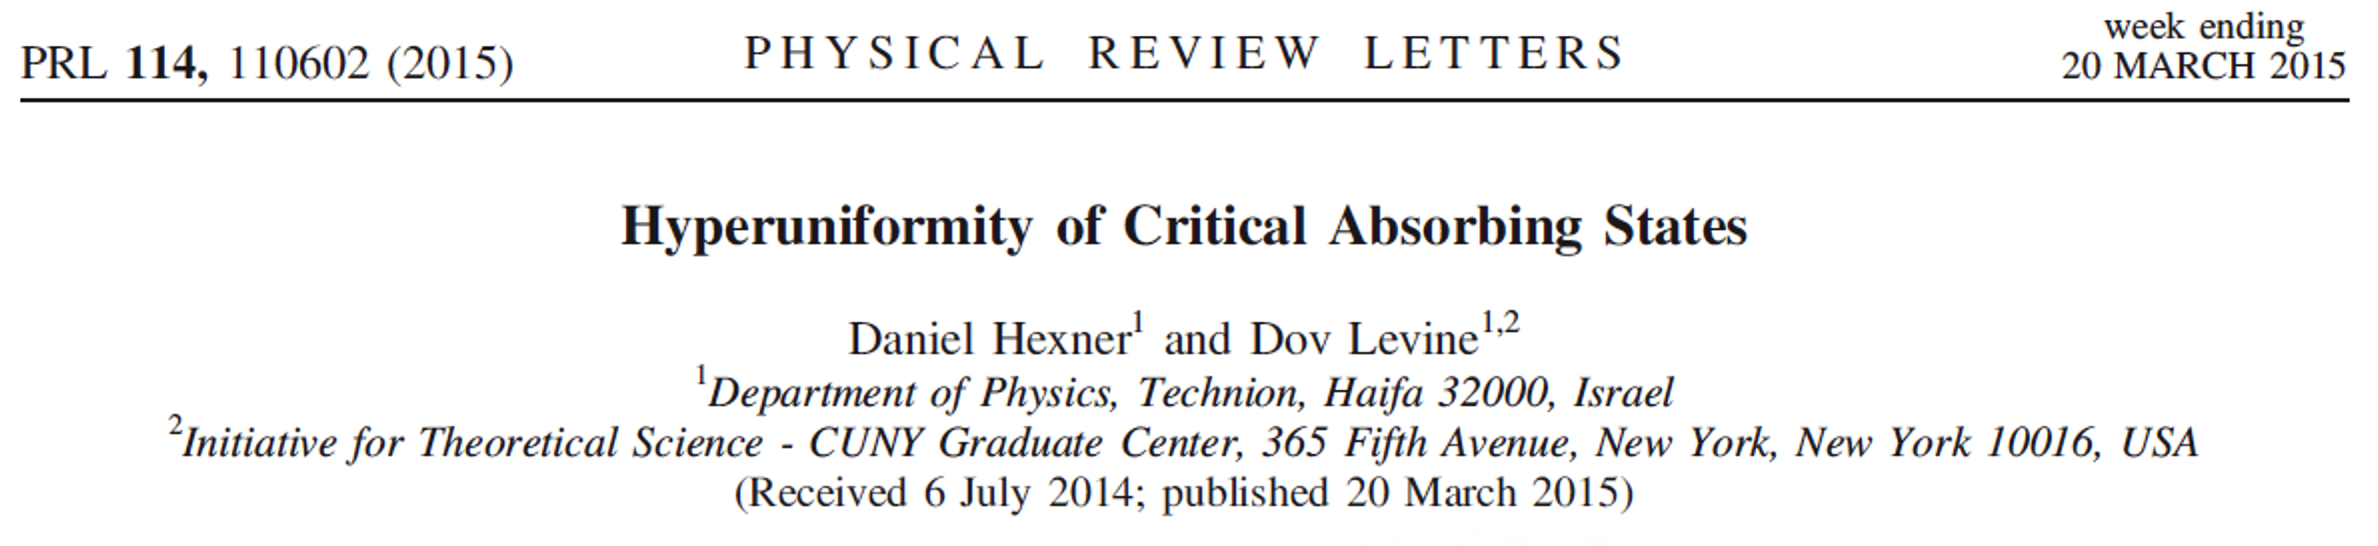
\includegraphics[scale=0.2]{images/p2.png}}
Abstract:
\begin{enumerate}[]
\item The properties of the absorbing states of nonequilibrium models belonging to $\textbf{the conserved directed percolation universality class}$ are studied. (Tips: 相变过程中,临界指数往往具有普适性 (universality):相同维数下,若观测到的属于相同的普适类)
\item At the critical point, the absorbing states are $\textbf{hyperuniform}$, exhibiting anomalously small density fluctuations.
\end{enumerate}
\end{frame}

\begin{frame}{References 03}
\centerline{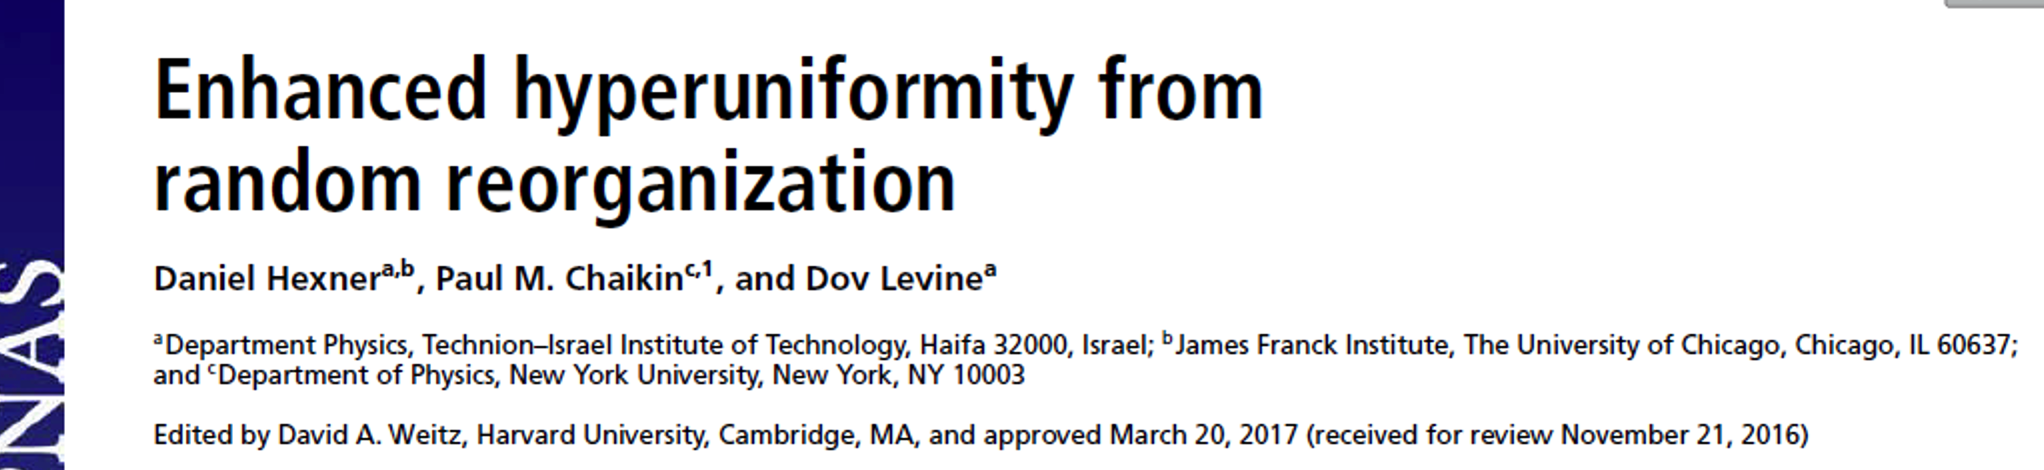
\includegraphics[scale=0.2]{images/p3.png}}
Abstract:
\begin{enumerate}[]
\item Above a critical particle density $\rho_{\mathrm{C}}$, the
system evolves forever, never finding a configuration where no
particles overlap. Below $\rho_{\mathrm{C}}$, however, it eventually finds such a
state, and stops evolving. 
\item This “absorbing state” is $\textbf{hyperuniform}$
up to a length scale $\xi$, which diverges at $\rho_{\mathrm{C}}$.
\end{enumerate}
\end{frame}

\begin{frame}{References 04}
\centerline{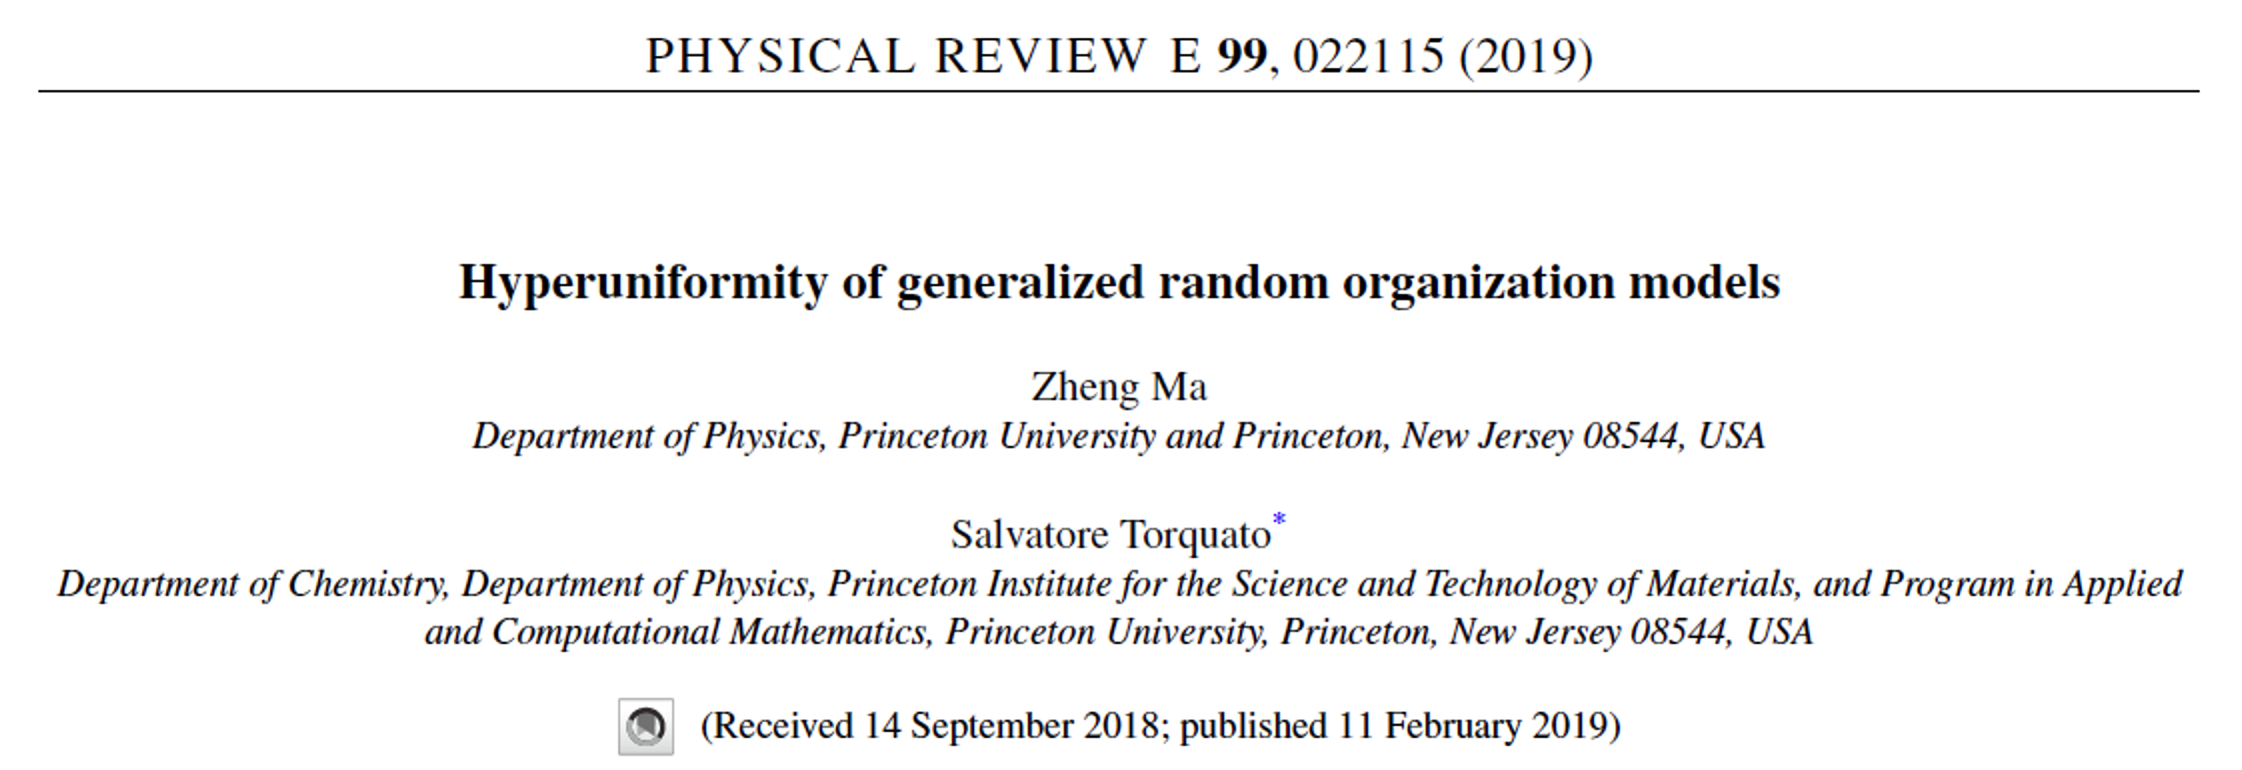
\includegraphics[scale=0.2]{images/p4.png}}
Abstract:
\begin{enumerate}[]
\item Here we investigate to what extent hyperuniformity is preserved when the model is generalized to $\textbf{particles with a size distribution and/or nonspherical shapes}$.
\item Our results suggest that general particle systems subject to random organization can be a robust way to fabricate a wide class of hyperuniform states of matter by tuning the structures via different particle-size and -shape distributions.
\end{enumerate}
\end{frame}

\begin{frame}{References 05}
\centerline{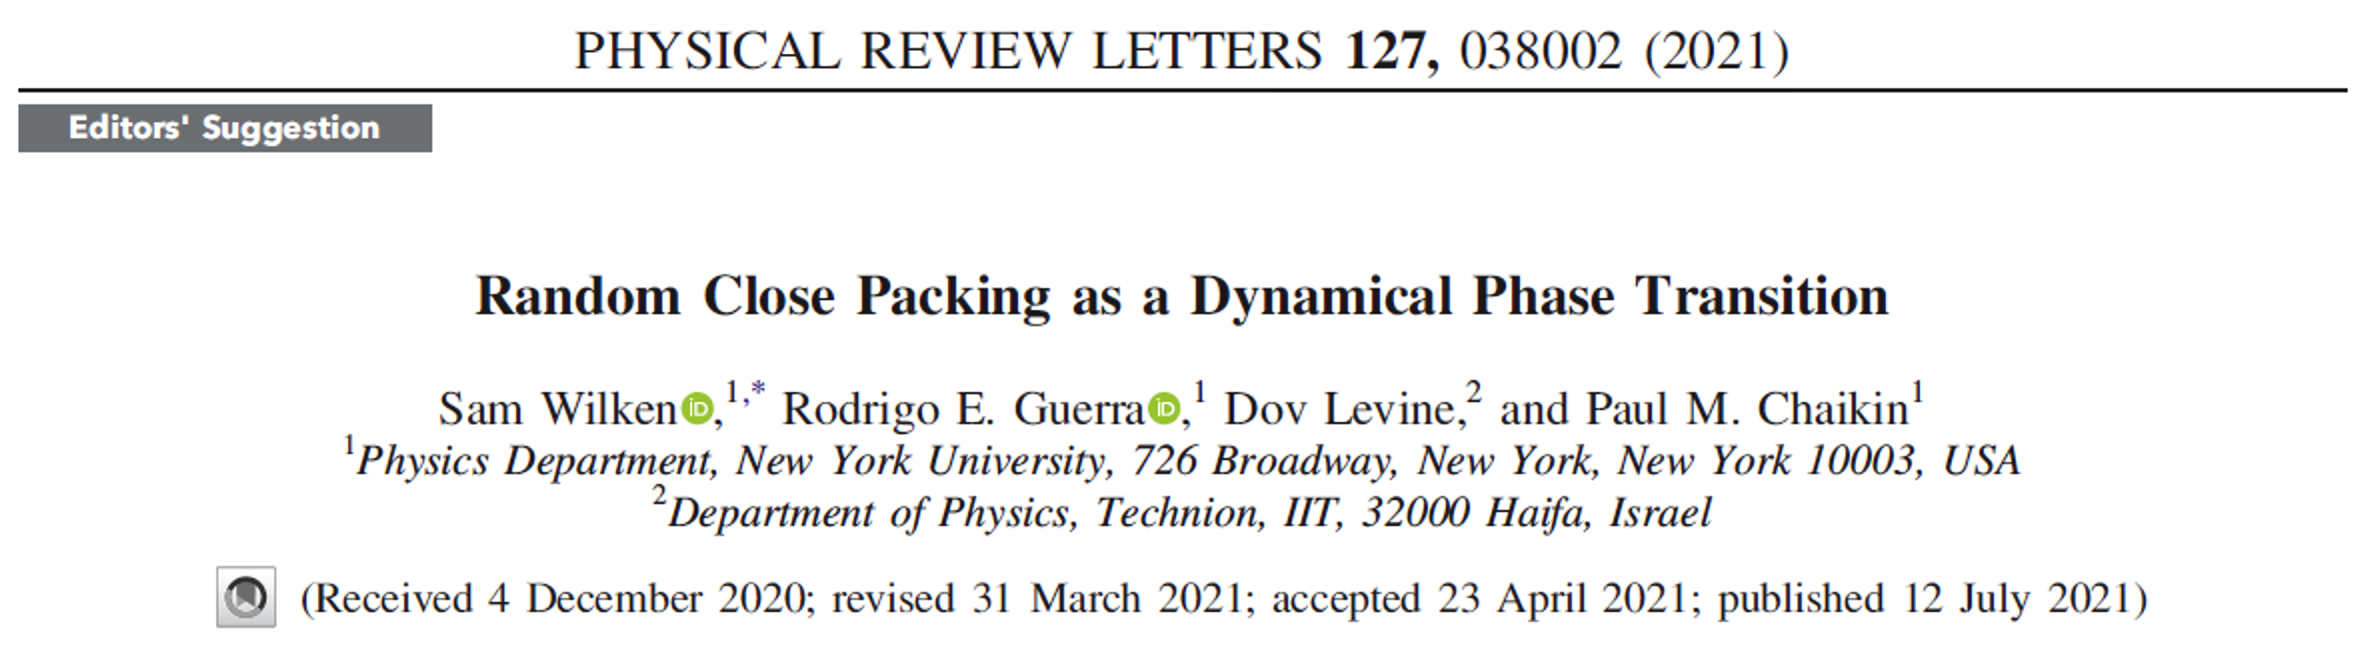
\includegraphics[scale=0.2]{images/p5.png}}
Abstract:
\begin{enumerate}[]
\item We introduce $\textbf{a simple absorbing-state model}$, biased random organization (BRO), which
exhibits a Manna class dynamical phase transition between absorbing and active states.
\item The configurations we obtain from BRO appear to be $\textbf{structurally identical to RCP configurations}$ from
other protocols.
\end{enumerate}
\end{frame}




\begin{frame}{Biased random organization}

\begin{columns}
\begin{column}{0.5\textwidth}
\centerline{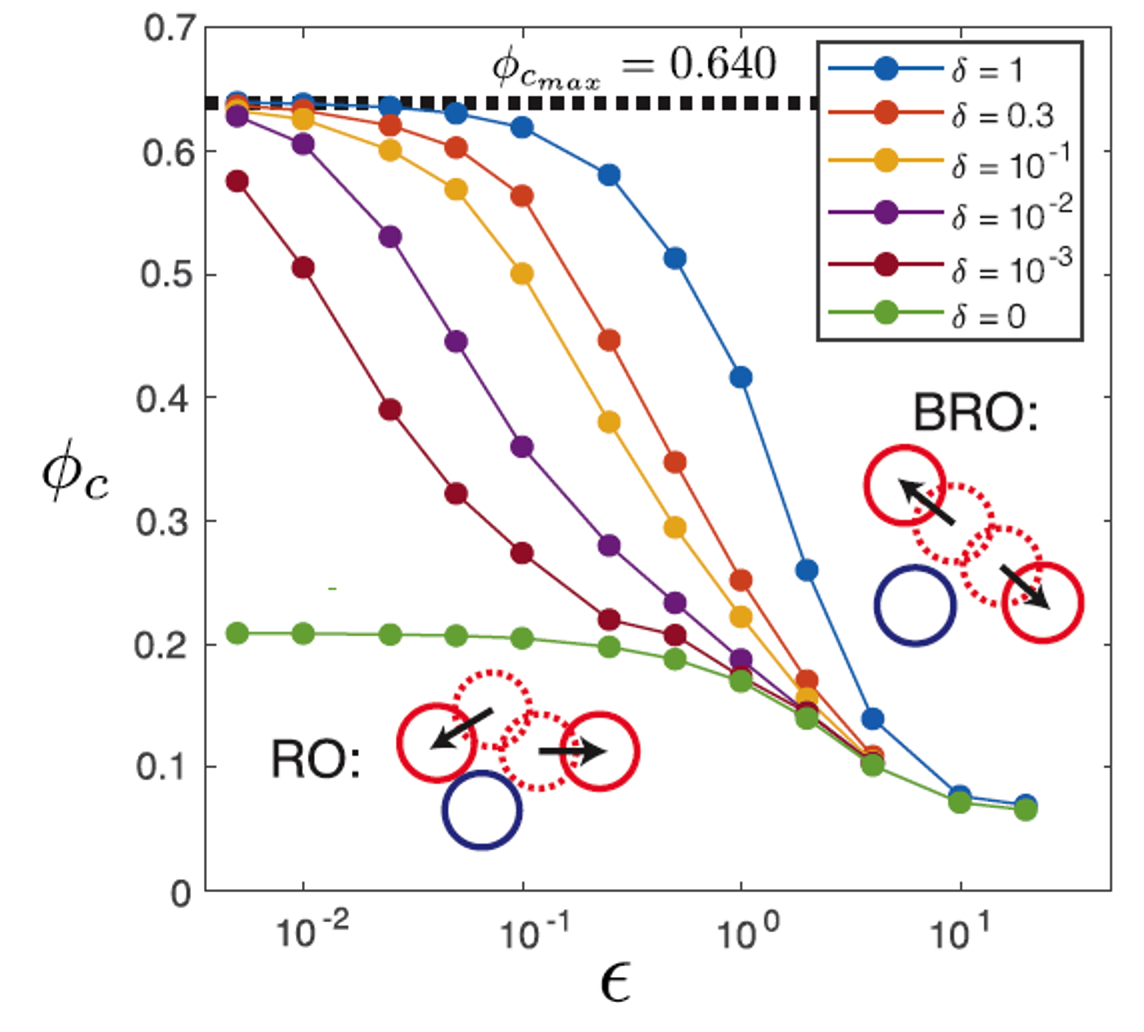
\includegraphics[scale=0.2]{images/p6.png}}
\centerline{$\textbf{The critical states of BRO are RCP configurations.}$}
\end{column}

\begin{column}{0.5\textwidth}
\
\newline\\
\setlength{\parindent}{2em}系统中的颗粒被分为active与inactive两类,对于inactive颗粒,给予两部分位移(描述颗粒碰撞):
\begin{enumerate}
\item 幅值(magnitude)为$\sqrt{\delta} \epsilon$的排斥位移(沿质心连线方向);
\item 幅值为$\sqrt{1-\delta} \epsilon$的随机方向位移。
\end{enumerate}
其中$\epsilon$以颗粒半径为单位。
\
\newline\\
特别地,当$\delta=0$时,模型退化为random organization.

\end{column}
\end{columns}
\end{frame}

\begin{frame}{Random organization}
\begin{columns}
\begin{column}{0.5\textwidth}
\centerline{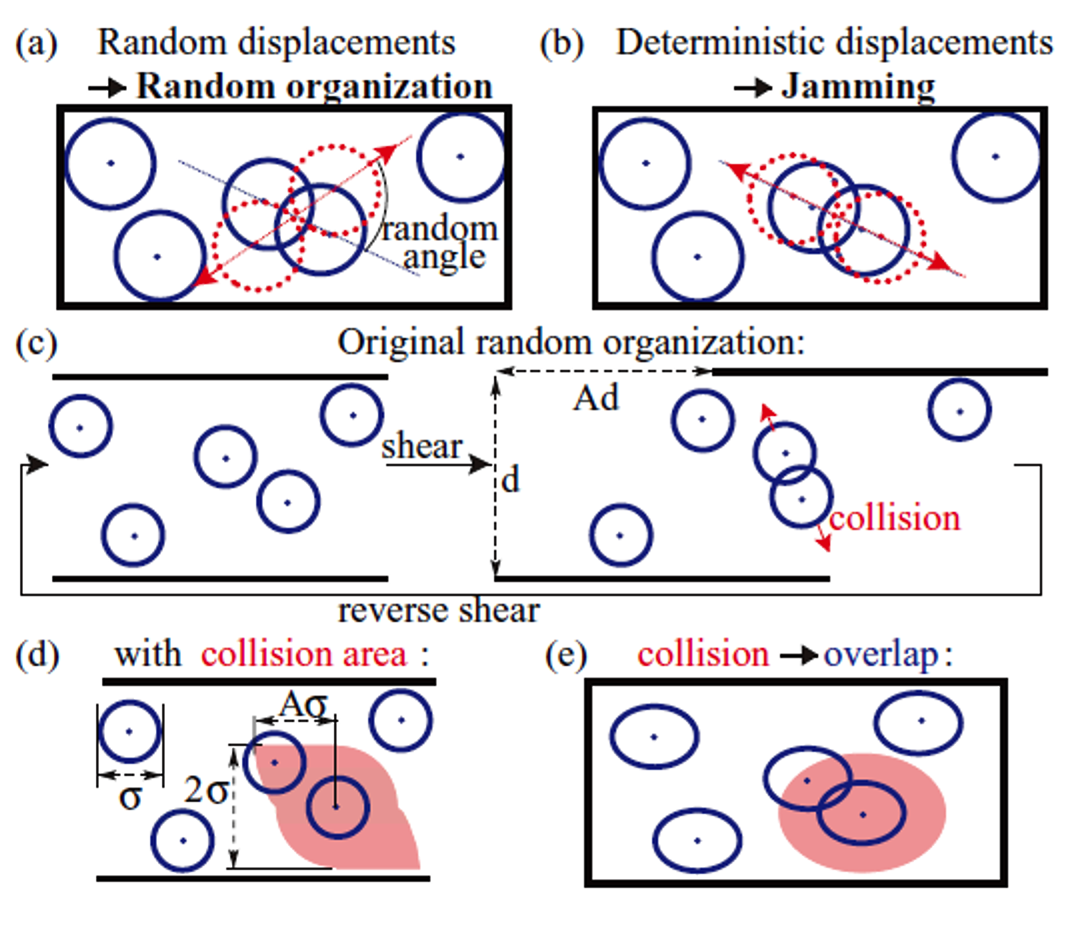
\includegraphics[scale=0.2]{images/p7.png}}
\end{column}

\begin{column}{0.5\textwidth}
\
\newline\\
\setlength{\parindent}{2em}一种非平衡现象,表示可逆和不可逆动力学之间的转变,系统从而分为两相:
\begin{enumerate}[]
\item An active phase, where dynamics persist forever;\\
\item An absorbing phase, in which the system ceases to evolve (once they arrive at an
absorbing state, they can never get out).\\
\end{enumerate}
\
\newline\\
视$\phi$低于或高于$\phi_c$,active颗粒的最终个数分数要么是0,要么是稳定的正值。
\end{column}
\end{columns}
\end{frame}

\begin{frame}{Random organization transition}
\centerline{\includegraphics[scale=0.2]{images/p8.png}}
\end{frame}

\begin{frame}{Hyperuniformity}
\setlength{\parindent}{2em}For a system in $d$ dimensions, we characterize the
density fluctuations in a region of volume $V=\ell^{d}$ by
$$\sigma^{2}(\ell) \equiv\left\langle\rho^{2}(\ell)\right\rangle-\langle\rho(\ell)\rangle^{2} \propto \ell^{-\lambda}$$
where $\rho(\ell)$ is the number of particles in the region divided by $V$.
\newline\
\begin{enumerate}[]
\item Random systems, e.g., a Possion process: $\lambda=d$.
\item Systems whose fluctuations decay faster with $d<\lambda \leq d+1$ are called hyperuniform (the larger $\lambda$, the more uniform).
\item For hyperuniform systems,
$S(k \rightarrow 0)=\frac{\left\langle N^{2}\right\rangle-\langle N\rangle^{2}}{\langle N\rangle} \rightarrow 0$.
\end{enumerate}
\
\newline\\
A hyperuniform state is achievable when the system goes through an absorbing phase transition to a critical state.
\end{frame}

\begin{frame}{Appendix}
\setlength{\parindent}{2em}We recall that for hyperuniform systems, 
$$S(\mathbf{k}) \sim|\mathbf{k}|^{\alpha} \quad(|\mathbf{k}| \rightarrow 0)$$
and the local number variance depends on the value of the exponent $\alpha$ as follows
$$\sigma_{N}^{2}(R) \sim \begin{cases}R^{d-1}, & \alpha>1 \quad \text { (CLASS I) } \\ R^{d-1} \ln R, \quad \alpha=1 & \text { (CLASS II) } \\ R^{d-\alpha}, \quad 0<\alpha<1 & \text { (CLASS III) }\end{cases}$$

\columnseprule=1pt         % 实现插入分隔线
\begin{multicols}{2} % 分两栏 若花括号中为3则是分三列
\centerline{\includegraphics[scale=0.18]{images/p9.png}}
\centerline{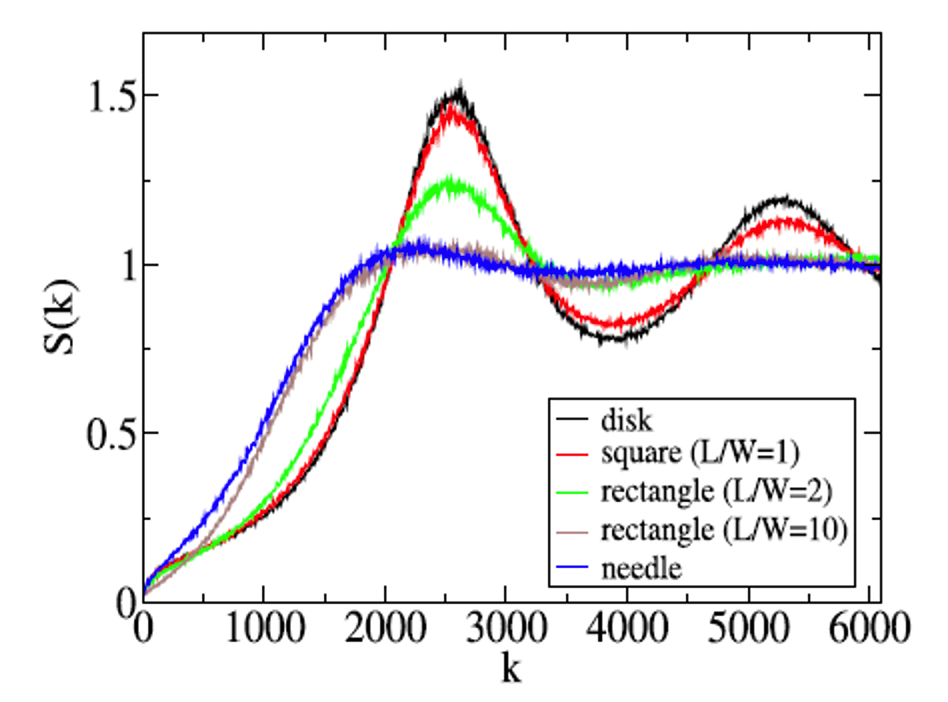
\includegraphics[scale=0.18]{images/p10.png}}
\end{multicols}

\end{frame}

\begin{frame}{Conserved lattice gas (CLG)}
\begin{columns}
\begin{column}{0.5\textwidth}
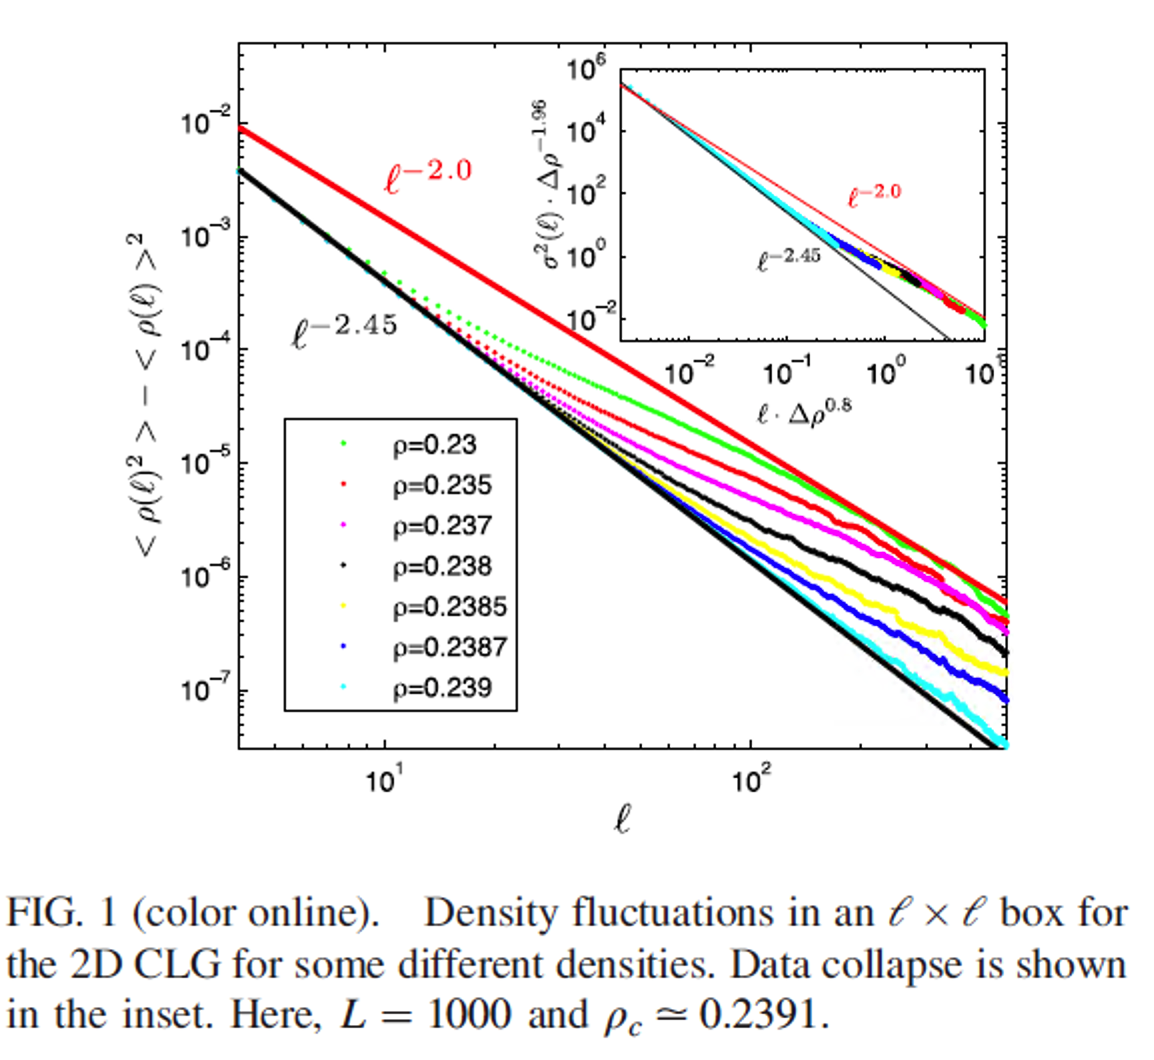
\includegraphics[scale=0.2]{images/1.jpg}
\end{column}

\begin{column}{0.5\textwidth}
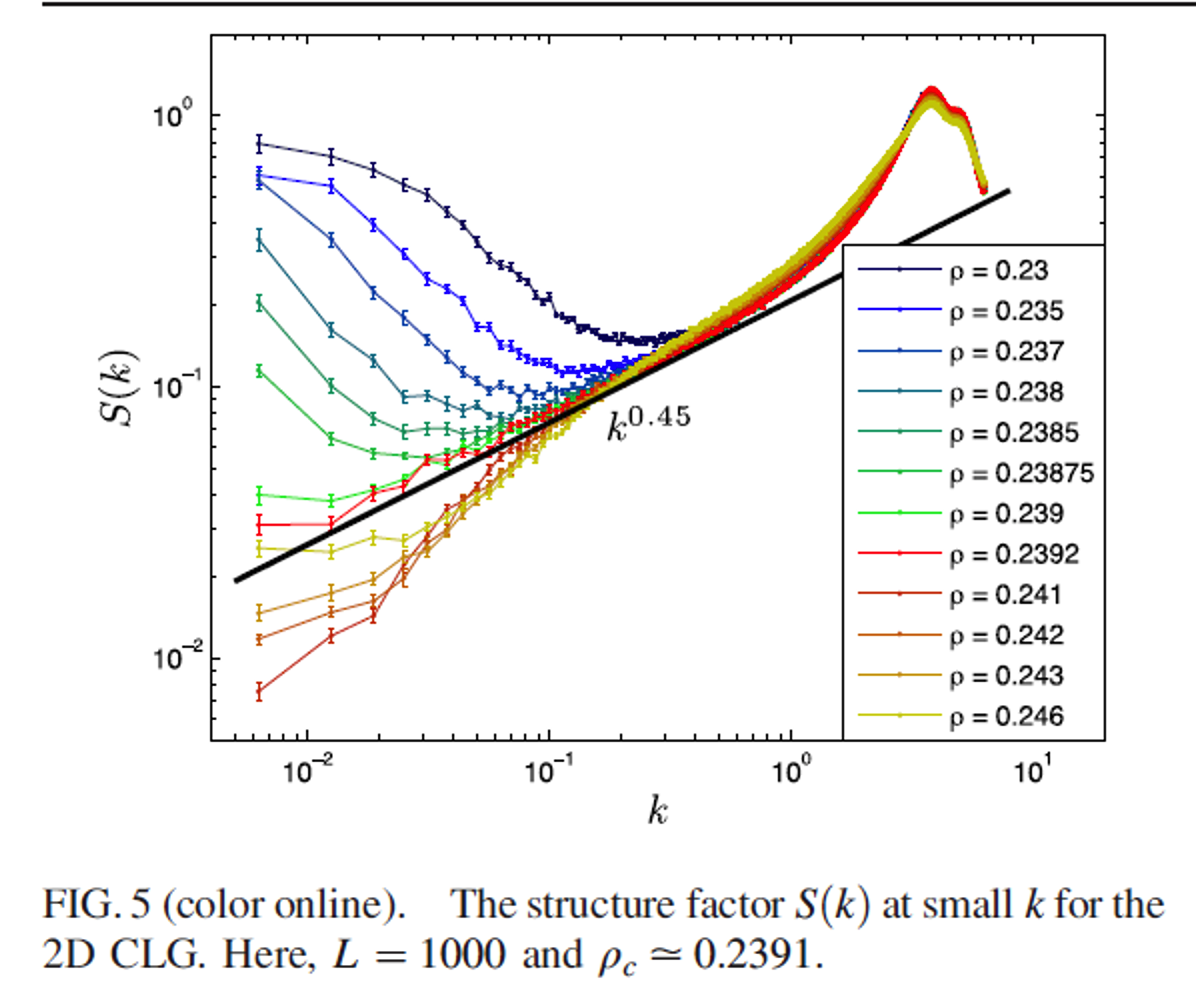
\includegraphics[scale=0.2]{images/5.jpg}
\end{column}
\end{columns}
\end{frame}

\begin{frame}{BRO与RCP}
\centerline{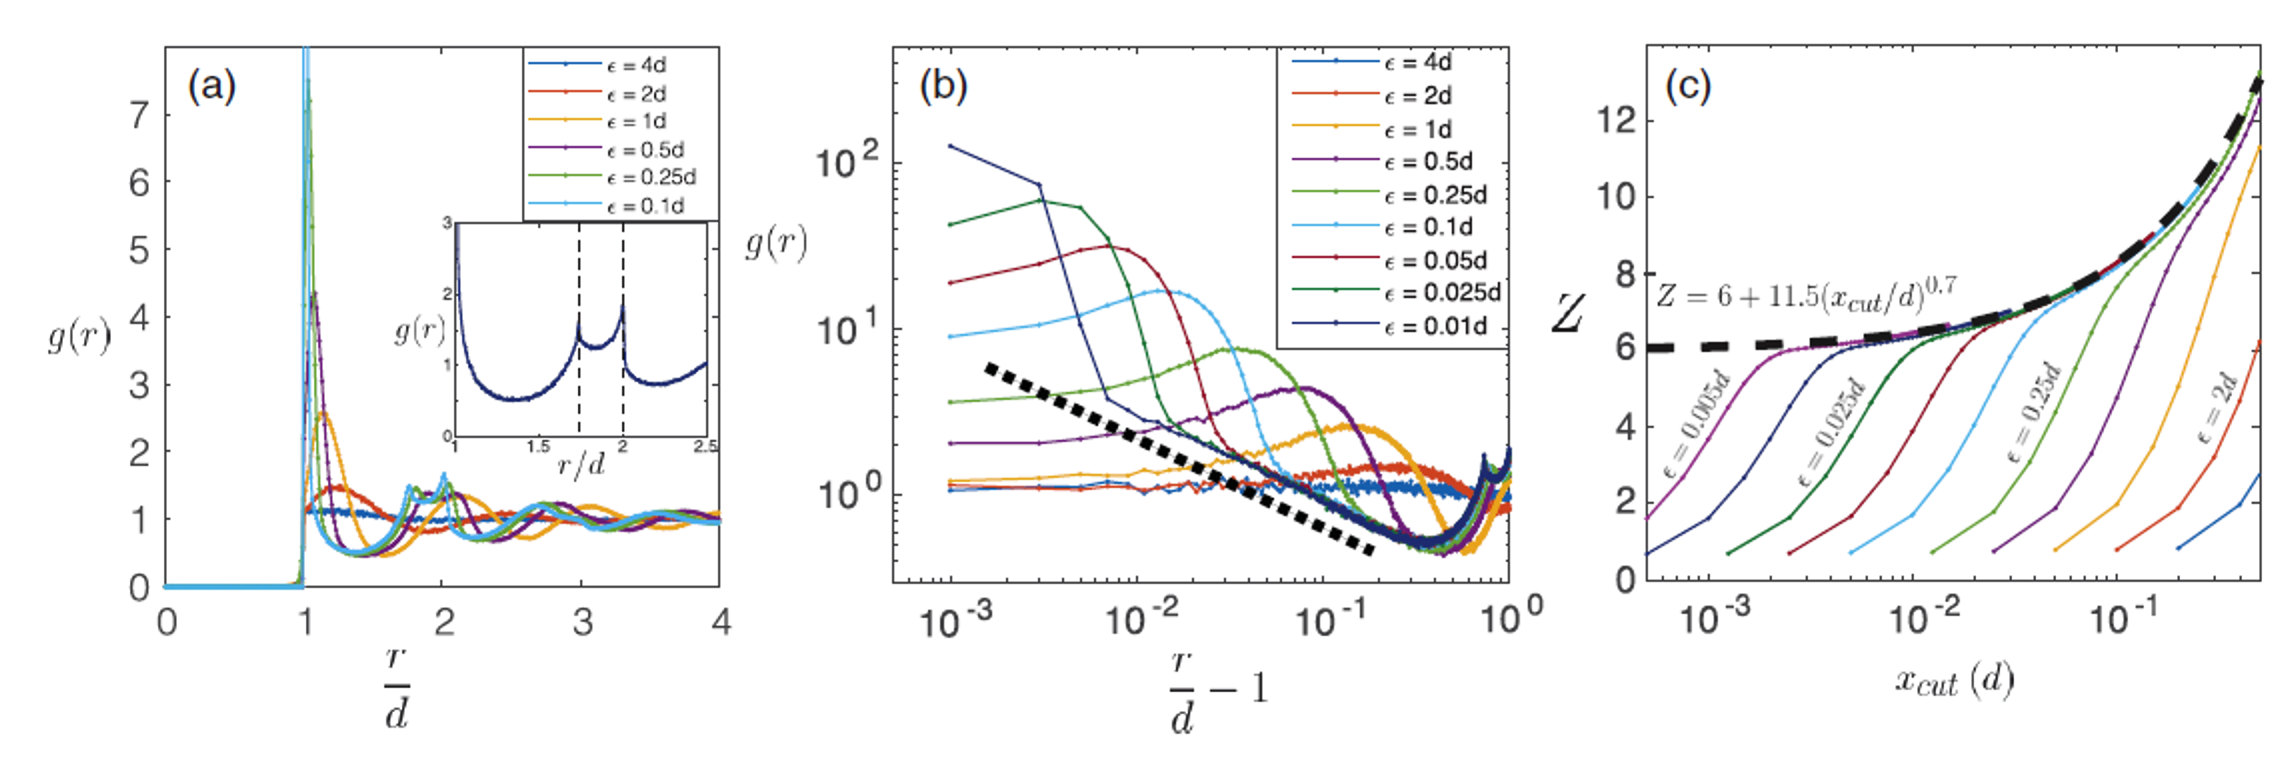
\includegraphics[scale=0.2]{images/p11.png}}
$$g(r) \sim(r / d-1)^{-1 / 2}$$
$$Z\left(x_{\mathrm{cut}}\right)=\left(24 \phi_{c}\right) / d^{3} \int_{d}^{d+x_{\text {cut }}} g(r) r^{2} d r$$
\centerline{Random close packing structure at $\phi_{c}(\epsilon \rightarrow 0)$ for $\delta=1$.}
\end{frame}

\begin{frame}{BRO与RCP}
\begin{columns}
\begin{column}{0.5\textwidth}
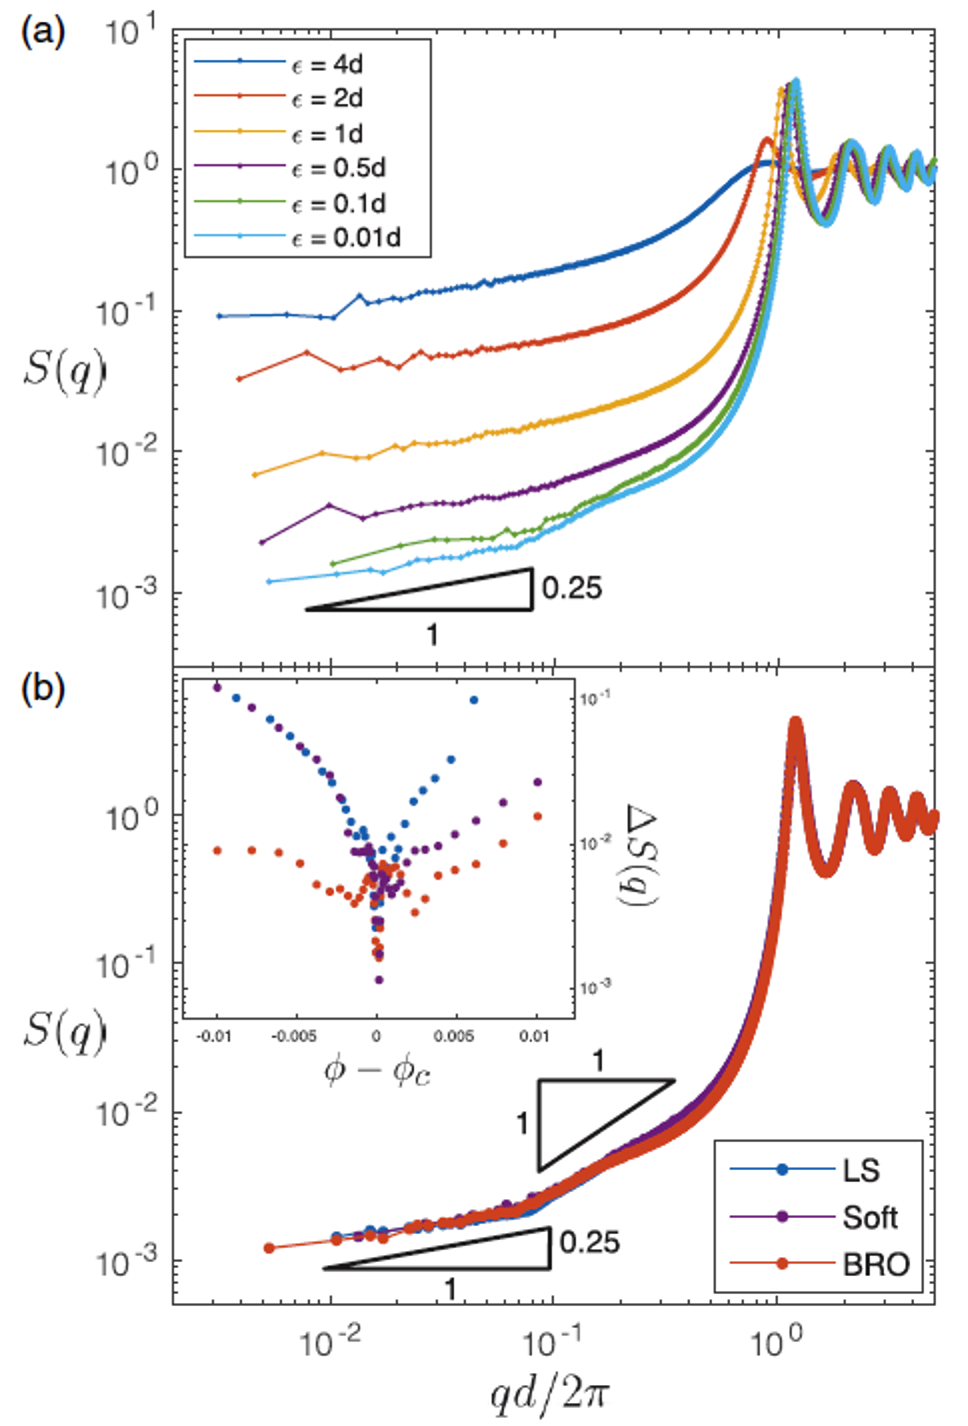
\includegraphics[scale=0.2]{images/p12.png}
\end{column}

\begin{column}{0.5\textwidth}
\begin{enumerate}[]
\item We find hyperuniform scaling $S(q \rightarrow 0) \sim q^{\alpha}$ with $\alpha \approx 0.25$ for all critical structures.
\item $$\Delta S(q)=\int_{0}^{5 \frac{2 \pi}{d}}\left|S(q, \phi) / S\left(q, \phi_{c}\right)-1\right| d q$$
BRO is not a disguised form of a previously studied model.
\item Why the BRO critical point is seemingly coincident at $\phi_{RCP}$ with the results of previous protocols?
\end{enumerate}
\end{column}
\end{columns}
\end{frame}

\section{Polytetrahedral aggregates (多四面体集合)}
\begin{frame}{References 01}
\centerline{\includegraphics[scale=0.2]{images/pp1.png}}
Abstract:
\begin{enumerate}[]
\item The number of spheres participating in
such polytetrahedral configurations increases with densification of the packing, and $\textbf{at the Bernal's limiting density (the packing fraction around 0.64) all}$ $\textbf{spheres of the packing become involved in such tetrahedra}$.
\end{enumerate}
\end{frame}

\begin{frame}{References 02}
\centerline{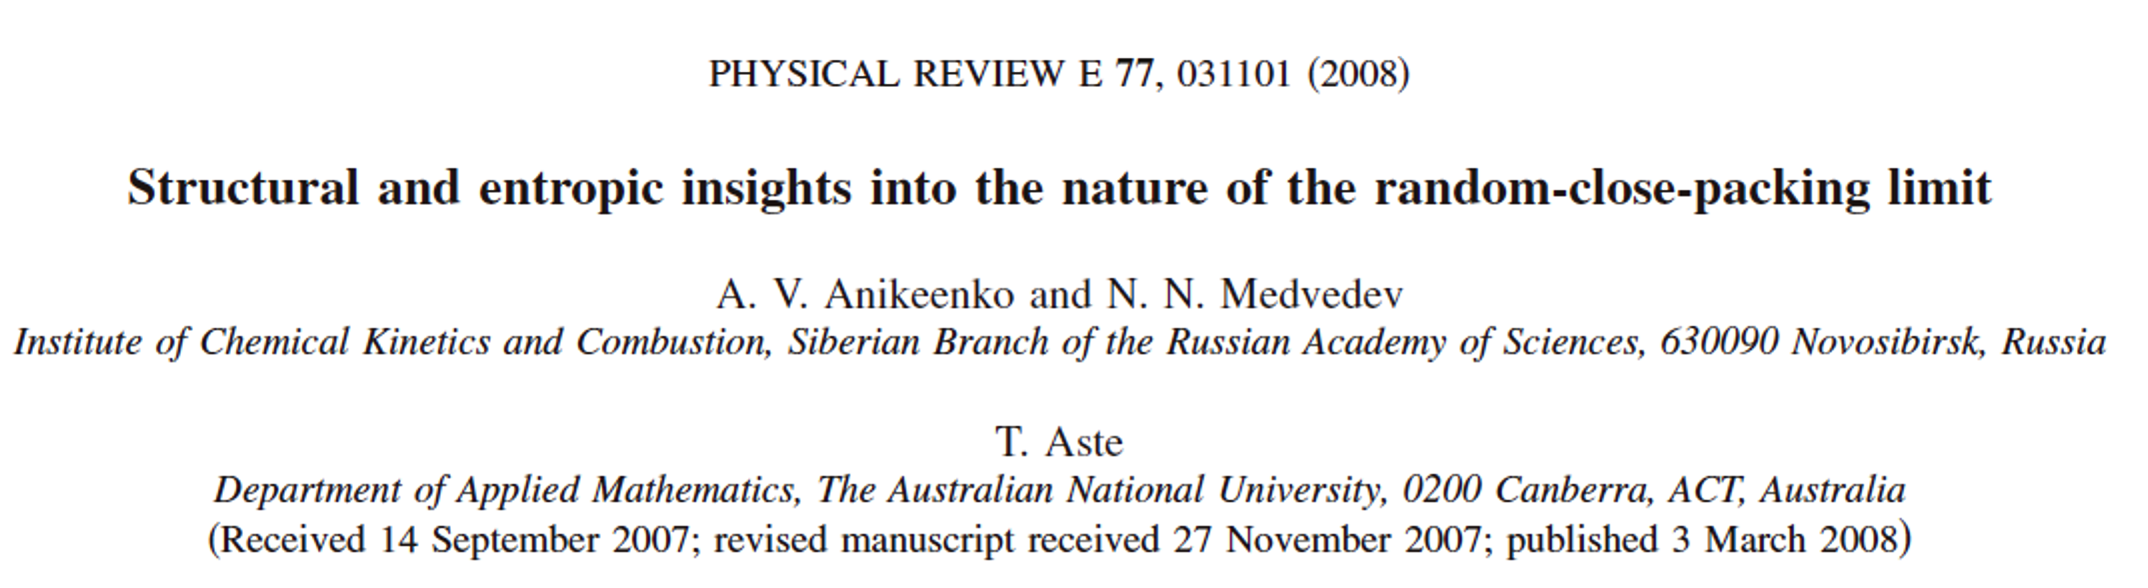
\includegraphics[scale=0.2]{images/pp2.png}}
Abstract:
\begin{enumerate}[]
\item At this limit the fraction of aggregate ''polytetrahedra'' structures (made of quasiperfect tetrahedra which share a common triangular face) reaches it maximal extension involving all the spheres.
\item Above the RCP limit the polytetrahedral structure gets rapidly disassembled.
\end{enumerate}
\end{frame}

\begin{frame}{References 03}
\centerline{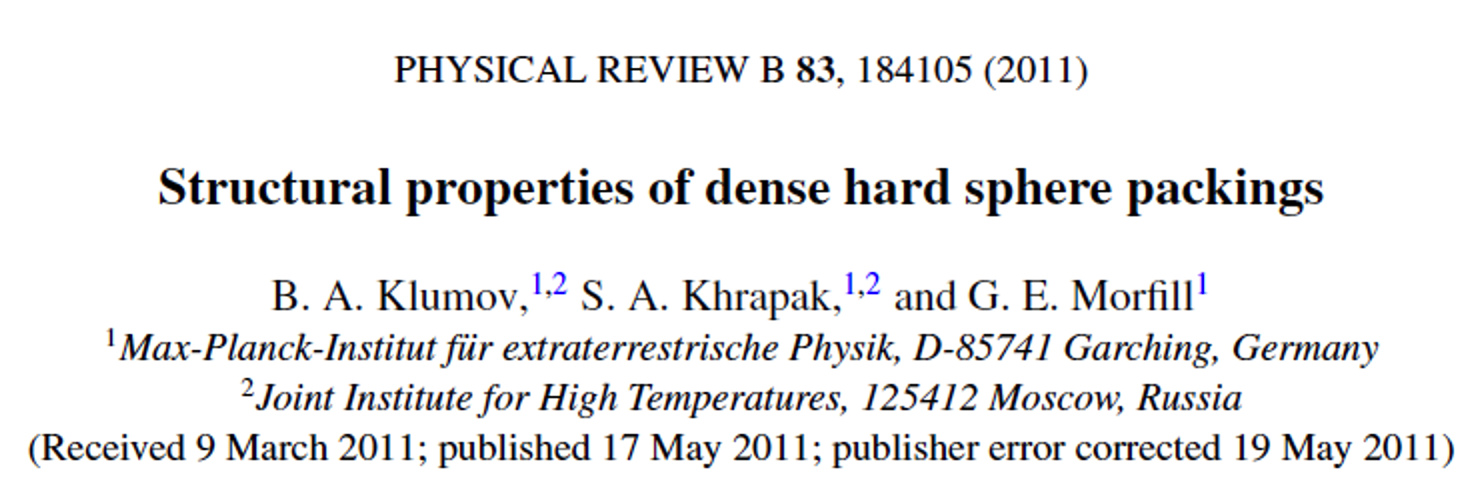
\includegraphics[scale=0.2]{images/pp3.png}}
Abstract:
\begin{enumerate}[]
\item It is shown that an increase in the packing fraction of the
crystallized HS system first results in the transformation of the individual crystalline clusters into the global
three-dimensional crystalline structure, which, upon further densification, transforms into alternating $\textbf{planar layers}$ formed by different lattice types.
\end{enumerate}
\end{frame}

\begin{frame}{Delaunay simplex}
\begin{columns}
\begin{column}{0.5\textwidth}
\begin{enumerate}[]
\item The maximal simplex edge length of a simplex (in units of the diameter of the sphere): $$e_{max}$$
\item The difference of the maximal edge lengths from unit: $$\delta=e_{\max }-1$$
\item ''Quasiregular tetrahedra'' (or simply tetrahedra): those simplexes with $\delta <0.255$
\item 通过引入更多判据,还可以定义一个 "quasiperfect tetrahedra",此处不赘述
\end{enumerate}
\end{column}

\begin{column}{0.5\textwidth}
\centerline{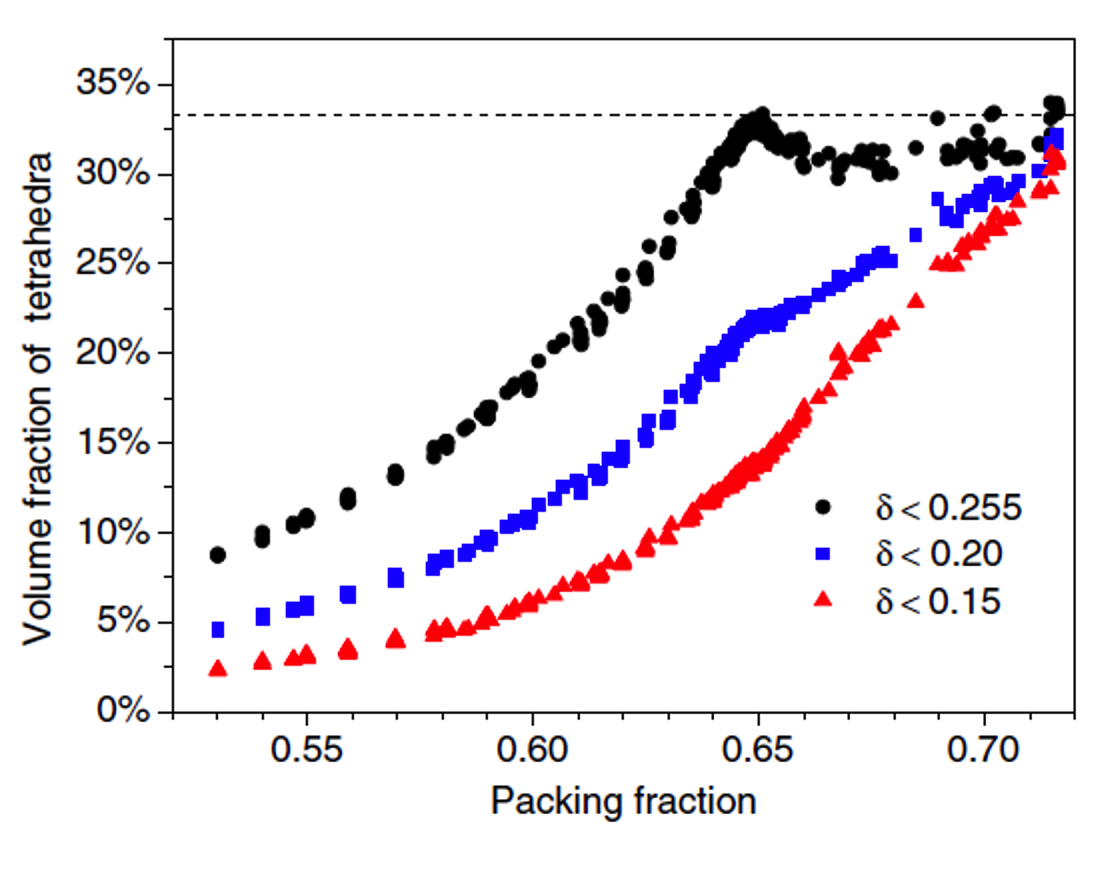
\includegraphics[scale=0.2]{images/pp4.png}}
\centerline{1/3: fcc and hcp}
\end{column}
\end{columns}
\end{frame}

\begin{frame}{Polytetrahedral aggregates}
\begin{columns}
\begin{column}{0.5\textwidth}
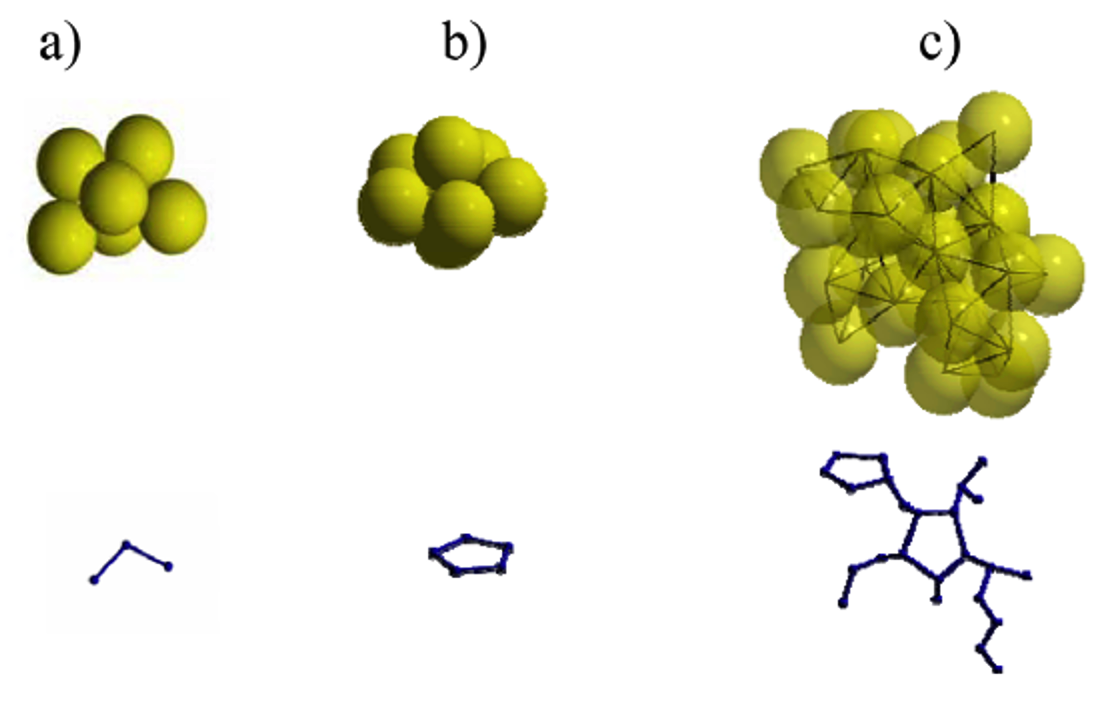
\includegraphics[scale=0.2]{images/pp5.png}
\centerline{With face-adjacent tetrahedra}
\end{column}

\begin{column}{0.5\textwidth}
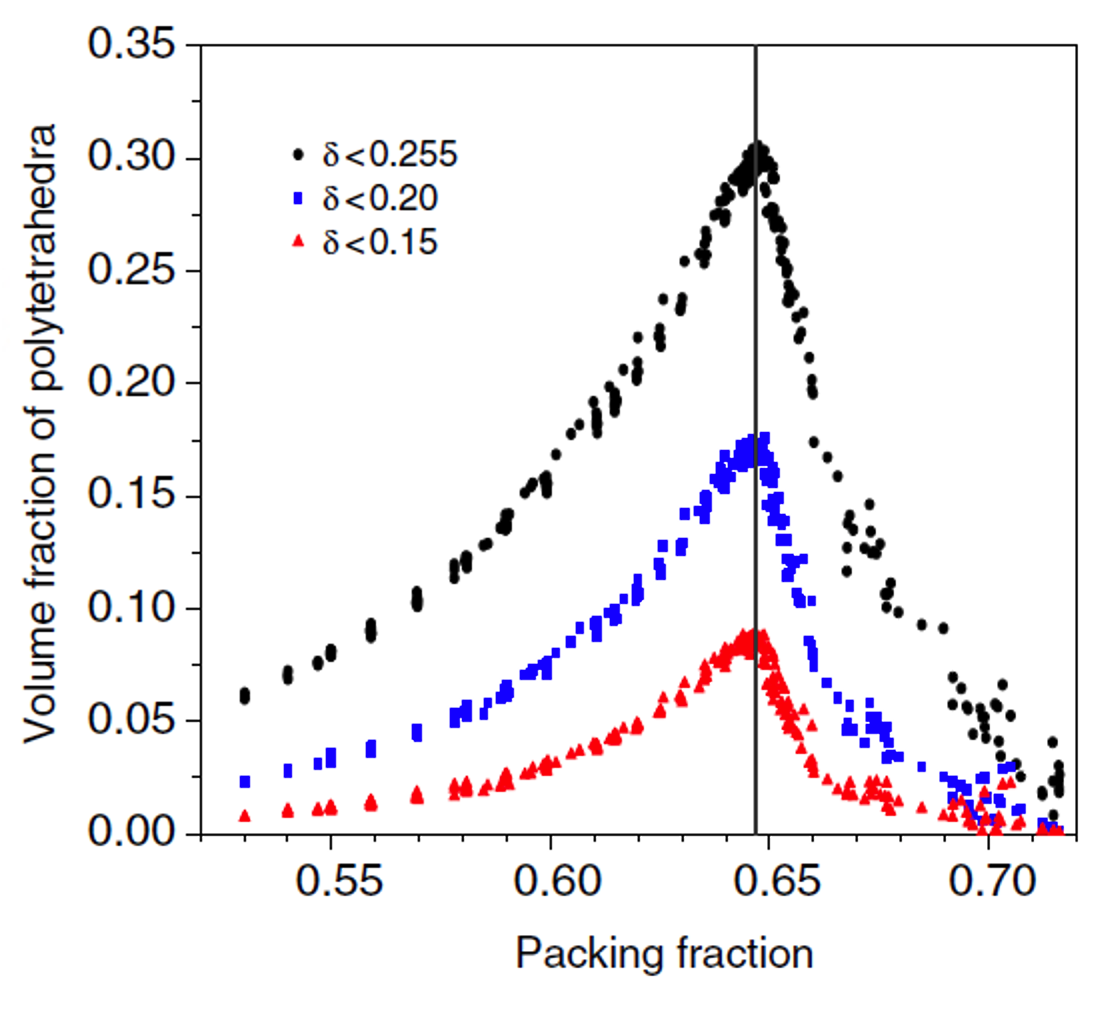
\includegraphics[scale=0.2]{images/pp6.png}
\end{column}
\end{columns}
The question then arises why this principle stops working for high density?
\end{frame}

\begin{frame}{Polytetrahedral aggregates}
\begin{columns}
\begin{column}{0.5\textwidth}
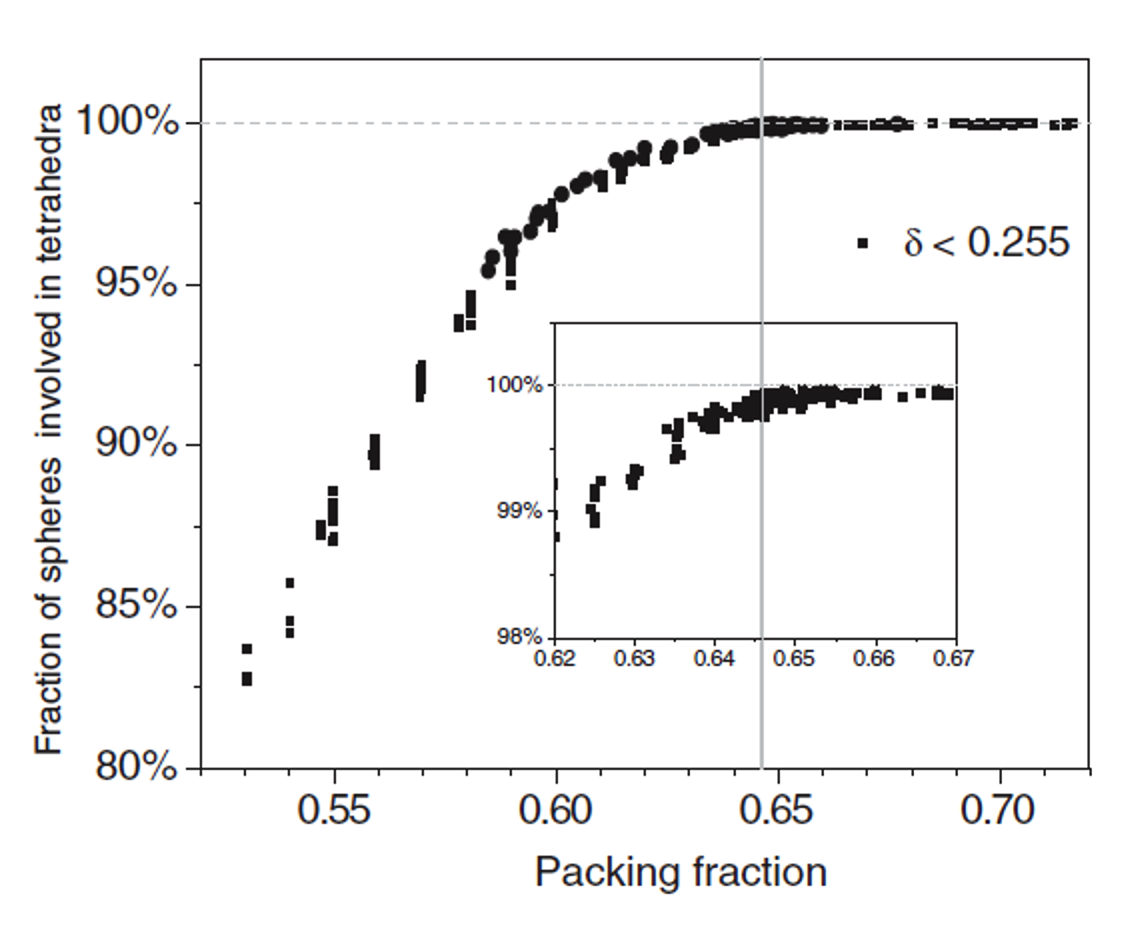
\includegraphics[scale=0.2]{images/pp7.png}
\end{column}

\begin{column}{0.5\textwidth}
\begin{enumerate}
\item Upon reaching this density only a very
small fraction of spheres avoid involvement in tetrahedra.
\item After all spheres of the system
have been involved, a further densification would require
another mechanism to increase the density of the packing.
\end{enumerate}
\end{column}
\end{columns}
\end{frame}

\begin{frame}{Entropic characterization}
\begin{columns}
\begin{column}{0.5\textwidth}
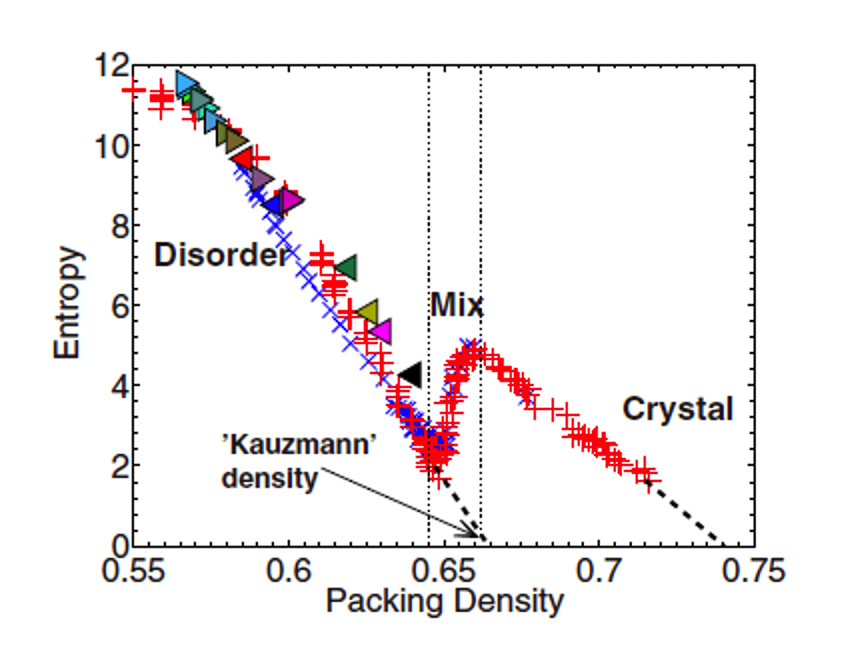
\includegraphics[scale=0.3]{images/pp8.png}
\end{column}

\begin{column}{0.5\textwidth}
\begin{enumerate}[]
\item 颗粒统计力学中,体积即能量,则某构型占据体积V的概率分布为:
$$p(V)=\frac{\Omega(V)}{\Omega(\chi)} \exp \left(-\frac{V}{\chi}\right)$$
\item 系统的熵为:
$$S=k\left[1+\ln \left(\frac{\bar{V}-V_{\min }}{k \Lambda^{3}}\right)\right]$$
\item Above the density of 0.646, it becomes more probable to
produce phase-separated mixtures of crystalline and disordered
phases.
\end{enumerate}
\end{column}
\end{columns}
\end{frame}

\begin{frame}{Sensitive order parameter}
\begin{columns}
\begin{column}{0.5\textwidth}
\centerline{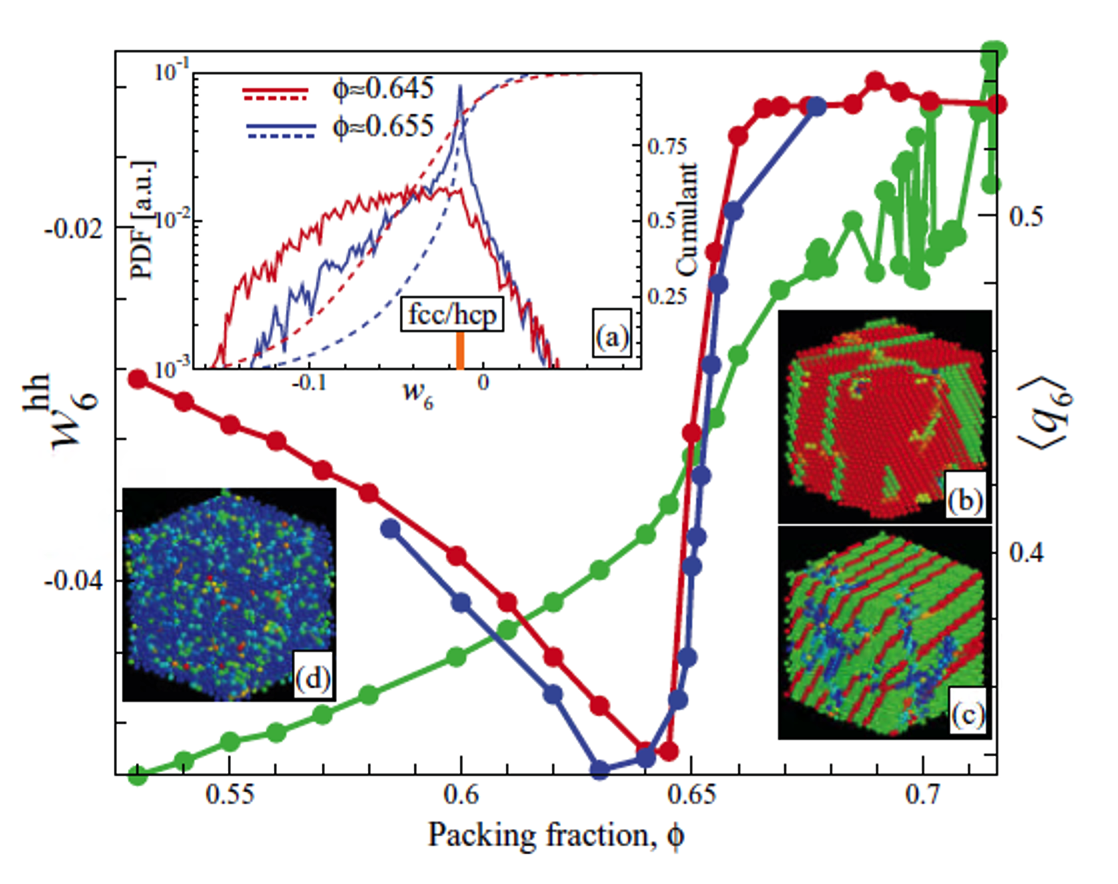
\includegraphics[scale=0.2]{images/pp9.png}}
\begin{enumerate}
\item Order parameter $w_{6}^{\mathrm{hh}}$ (red and blue lines correspond
to JT and LS packing protocols, respectively)
\item The mean value of the rotational invariant $\left\langle q_{6}\right\rangle$ (green)
\end{enumerate}
\end{column}

\begin{column}{0.5\textwidth}
\centerline{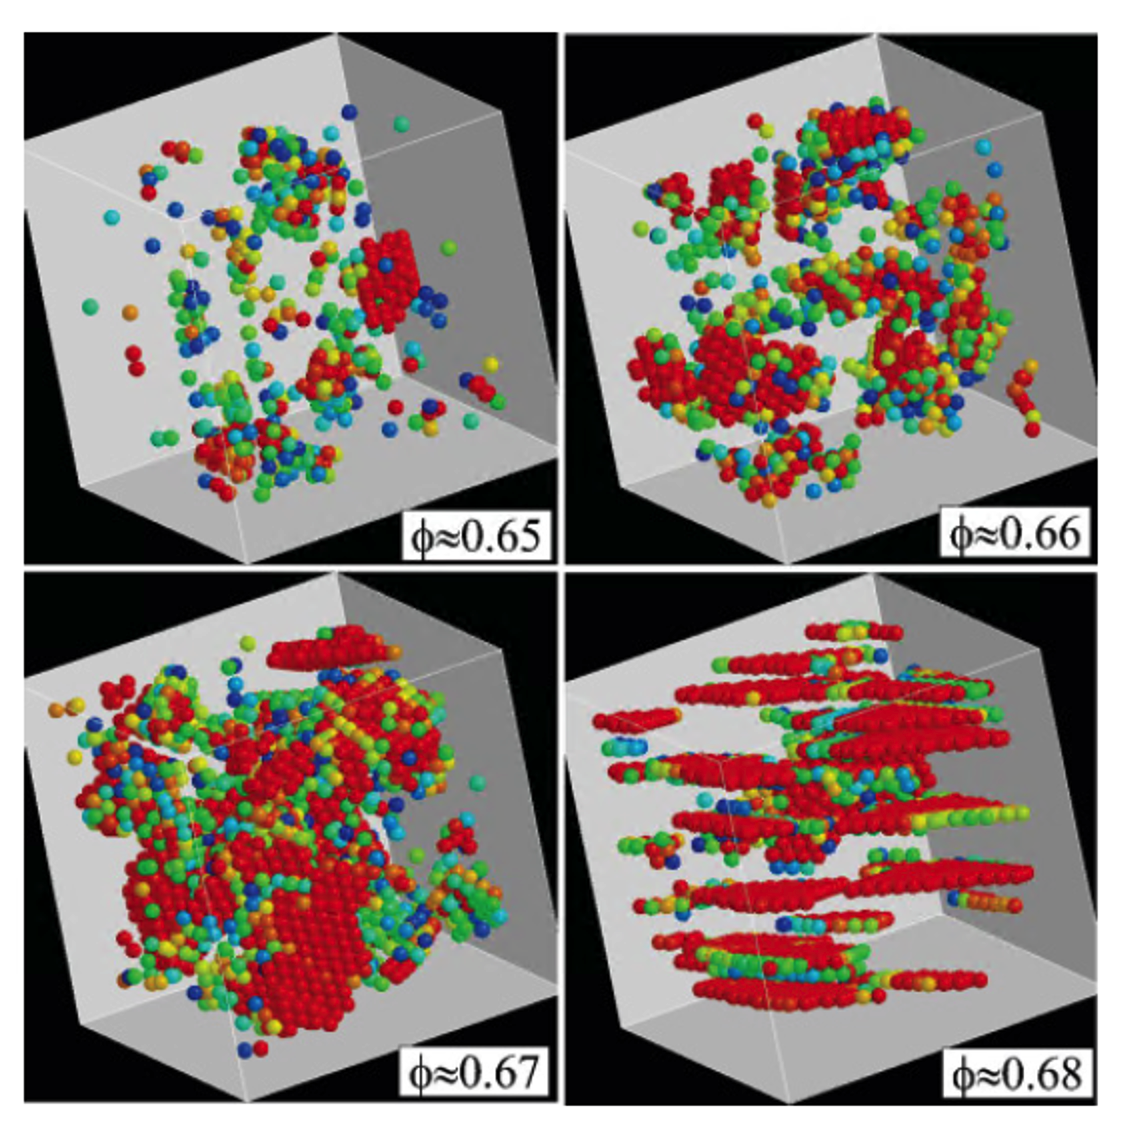
\includegraphics[scale=0.2]{images/pp10.png}}
\end{column}
\end{columns}
\end{frame}

\section{Extra}
\begin{frame}
\centerline{Thanks for listening!}
\end{frame}

\end{document}

